\documentclass{article}
\usepackage{tikz}
\usepackage{caption}

\begin{document}
\begin{figure}
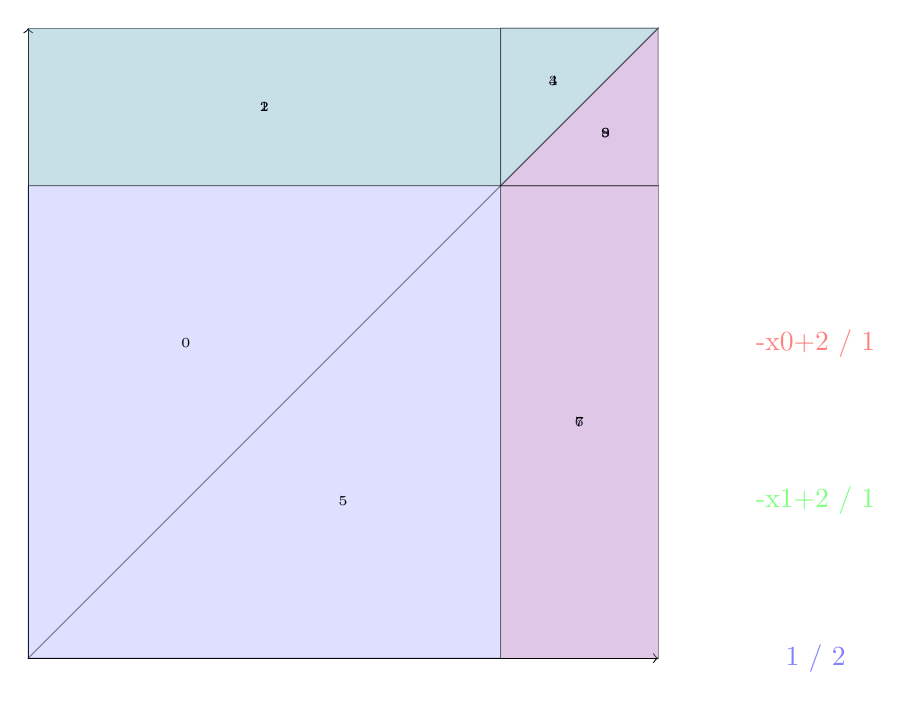
\begin{tikzpicture}[scale=4]
\draw[black,->] (0,0) -- (2,0);
\draw[black,->] (0,0) -- (0,2);
\draw[fill=blue!50, opacity=0.25] (0 / 2, 3 / 2) -- (3 / 2, 3 / 2) -- (0 / 1, 0 / 1) -- cycle;
\node at (3 / 6, 6 / 6) { \tiny{ 0 } };
\draw[fill=green!50, opacity=0.25] (0 / 1, 2 / 1) -- (3 / 2, 4 / 2) -- (3 / 2, 3 / 2) -- (0 / 2, 3 / 2) -- cycle;
\node at (6 / 8, 14 / 8) { \tiny{ 1 } };
\draw[fill=blue!50, opacity=0.25] (0 / 1, 2 / 1) -- (3 / 2, 4 / 2) -- (3 / 2, 3 / 2) -- (0 / 2, 3 / 2) -- cycle;
\node at (6 / 8, 14 / 8) { \tiny{ 2 } };
\draw[fill=green!50, opacity=0.25] (3 / 2, 3 / 2) -- (3 / 2, 4 / 2) -- (2 / 1, 2 / 1) -- cycle;
\node at (10 / 6, 11 / 6) { \tiny{ 3 } };
\draw[fill=blue!50, opacity=0.25] (3 / 2, 3 / 2) -- (3 / 2, 4 / 2) -- (2 / 1, 2 / 1) -- cycle;
\node at (10 / 6, 11 / 6) { \tiny{ 4 } };
\draw[fill=blue!50, opacity=0.25] (0 / 1, 0 / 1) -- (3 / 2, 3 / 2) -- (3 / 2, 0 / 2) -- cycle;
\node at (6 / 6, 3 / 6) { \tiny{ 5 } };
\draw[fill=red!50, opacity=0.25] (3 / 2, 0 / 2) -- (3 / 2, 3 / 2) -- (4 / 2, 3 / 2) -- (2 / 1, 0 / 1) -- cycle;
\node at (14 / 8, 6 / 8) { \tiny{ 6 } };
\draw[fill=blue!50, opacity=0.25] (3 / 2, 0 / 2) -- (3 / 2, 3 / 2) -- (4 / 2, 3 / 2) -- (2 / 1, 0 / 1) -- cycle;
\node at (14 / 8, 6 / 8) { \tiny{ 7 } };
\draw[fill=red!50, opacity=0.25] (3 / 2, 3 / 2) -- (2 / 1, 2 / 1) -- (4 / 2, 3 / 2) -- cycle;
\node at (11 / 6, 10 / 6) { \tiny{ 8 } };
\draw[fill=blue!50, opacity=0.25] (3 / 2, 3 / 2) -- (2 / 1, 2 / 1) -- (4 / 2, 3 / 2) -- cycle;
\node at (11 / 6, 10 / 6) { \tiny{ 9 } };
\node[blue!50] at (2.5,0 / 2) { 1 / 2 };
\node[green!50] at (2.5,1 / 2) { -x1+2 / 1 };
\node[red!50] at (2.5,2 / 2) { -x0+2 / 1 };
\end{tikzpicture}
\caption{ test }
\end{figure}
\end{document}
